\newpage
\section{Technologierecherche}

Anforderungen in Teilfunktionen zerlegt:
\begin{itemize}
    \item Fortbewegung
    \item Antrieb
    \item Steuerung
    \item Orientierung
    \item Objekterkennung
    \item Wegfindung
    \item Sicherheit
    \item Energiequelle
    \item Hindernis Bewältigung
\end{itemize}

\subsection*{Überblick}

\scriptsize
\begin{longtable}{l@{\extracolsep{\fill}}p{2cm}p{2cm}p{4cm}p{1.5cm}lll}
%\toprule
\textbf{Dep.} & \textbf{Teilfunktion} & \textbf{Thema} &
\textbf{Beschreibung} & \textbf{Bewertung (0-10)} & \textbf{Quelle} & \textbf{Abfragedatum} &
\textbf{Wer}\tabularnewline
%\midrule
\endhead

M & Fortbewegung & Beweglichkeit & 2-Rad gegensinnig für 360° \newline Drehung im Stand & 8 & MC-Car & 01.10.2024 & Joel
\tabularnewline
M & Fortbewegung & Beweglichkeit & 4-Rad Differential steering / \newline skid steer & 8 & \href{https://en.wikipedia.org/wiki/Differential_steering}{Link} /\href{https://science.howstuffworks.com/transport/engines-equipment/skid-steer2.htm}{Link} & 03.10.2024 & Silas
\tabularnewline
M & Fortbewegung & Beweglichkeit & Omniwheels & 9 & \href{https://de.wikipedia.org/wiki/Allseitenrad}{Link} / \href{https://www.youtube.com/watch?v=wwQQnSWqB7A}{Link} & 03.10.2024 & Silas
\tabularnewline
M & Fortbewegung & Beweglichkeit & Knicklenkung & 4 & \href{https://de.wikipedia.org/wiki/Knicklenkung}{Link} & 03.10.2024 & Silas
\tabularnewline
M & Fortbewegung & Beweglichkeit & Achsschenkellenkung & 5 & \href{https://de.wikipedia.org/wiki/Achsschenkel#:~:text=Die%20Erfindung%20der%20Achsschenkellenkung%20bedeutete,wird%20bei%20Automobilen%20ausschlie%C3%9Flich%20verwendet.}{Link} & 03.10.2024 & Silas
\tabularnewline
M & Fortbewegung & Beweglichkeit & Drehschemellenkung & 5 & \href{https://www.staplerberater.de/auswahlkriterien/lenkungsarten}{Link} & 03.10.2024 & Silas
\tabularnewline
M & Fortbewegung & Beweglichkeit & Fahrzeug abbocken und an Stelle auf Drehkranz wenden & 6 & \href{https://www.kaiserkraft.ch/hubgeraete/hub-und-verladetische/auto-niveaugeraet-mit-drehscheibe/drehscheiben-1110-mm/p/M1142876/?articleNumber=118558&lang=de_CH&customerType=B2C&lang=&infinity=ict2~net~gaw~cmp~PM_DE-shopping24-Jarvis-0~ag~~ar~~kw~~mt~&gad_source=1&gclid=CjwKCAjwgfm3BhBeEiwAFfxrGxsQhJoEWwY3dNM_OYKFg2NOgoHXLP2OeyLmOZFTVnzHt7PvNpgCbhoCACQQAvD_BwE}{Link} & 03.10.2024 & Silas
\tabularnewline

E & Antrieb & Motor & Schrittmotor & 8 & \href{https://wiki.bu.ost.ch/infoportal/_media/hardware/sysp/bauteile/schrittmotor_kurz_erklaert_d.pdf}{Link} & 27.09.2024 & Thomas
\tabularnewline
E & Antrieb & Motor & DC Motor & 7 & \href{https://www.elektronikpraxis.de/dc-motoren-empirisch-und-theoretisch-berechnen-a-04bb230e718c01ace9dd584576d618a3/}{Link} & 27.09.2024 & Thomas
\tabularnewline
E & Antrieb & Motor & Brushless & 7 & \href{https://www.renesas.com/en/support/engineer-school/brushless-dc-motor-01-overview}{Link} & 27.09.2024 & Thomas
\tabularnewline

I & Steuerung & Hardware & Raspberry Pi & 8 & \href{https://www.raspberrypi.com/documentation/computers/raspberry-pi.html}{Link} & 29.09.2024 & Thomas
\tabularnewline
I & Steuerung & Hardware & Arduino & 5 & \href{https://arduino.cc/en/hardware#boards-1}{Link} & 29.09.2024 & Thomas
\tabularnewline
I & Steuerung & Hardware & Tiny & 8 & HSLU & 01.10.2024 & Joel
\tabularnewline
I & Steuerung & Hardware & ESP32 & 7 & \href{https://www.espressif.com/en/products/devkits/esp32-devkitc}{Link} & 03.10.2024 & Thomas
\tabularnewline

E & Orientierung & Sensorik & Infrarot & 5 & \href{https://www.elektronik-kompendium.de/sites/raspberry-pi/2802011.htm}{Link} & 27.09.2024 & Thomas
\tabularnewline
E & Orientierung & Sensorik & Ultraschall & 5 & \href{https://elektro.turanis.de/html/prj121/index.html}{Link} & 27.09.2024 & Thomas 
\tabularnewline
E & Orientierung & Sensorik & Encoder & 7 & \href{https://www.arrow.de/research-and-events/articles/rotary-encoders-how-to-pair-with-an-arduino-board}{Link} & 29.09.2024 & Thomas
\tabularnewline
E & Orientierung & Sensorik & Optischer Sensor & 5 & \href{https://global.sharp/products/device/lineup/data/pdf/datasheet/gp2y0e02a_e.pdf}{Link} & 01.10.2024 & Joel
\tabularnewline

I & Objekterkennung & Deep Learning & Deep Learning Frameworks & 7 &  \href{https://www.simplilearn.com/tutorials/deep-learning-tutorial/deep-learning-frameworks} {Link}&  27.09.2024 & Gian
\tabularnewline
I & Objekterkennung & Deep Learning & TensorFlow in 100 seconds & 10 &
\href{https://www.youtube.com/watch?v=i8NETqtGHms}{Link} & 29.09.2024 & Gian
\tabularnewline
I & Objekterkennung & Deep Learning & What is Object Detection? & 9 &
\href{https://www.ibm.com/topics/object-detection#:~:text=Object%20detection%20is%20a%20technique,imaging%20to%20self%2Ddriving%20cars.}{Link}
& 02.10.2024 & Gian
\tabularnewline
I & Objekterkennung & Deep Learning & Region Based CNN - Wikipedia &
\href{https://en.wikipedia.org/wiki/Region_Based_Convolutional_Neural_Networks}{Link}
& 6 & 02.10.2024 & Gian
\tabularnewline
I & Wegfindung & Algorithmus & Informationen über Wegfindung & \href{https://de.wikipedia.org/wiki/Pathfinding}{Link} & 8 & 02.10.2024 & Gian
\tabularnewline
I & Wegfindung & Test & Test & Test & Test & Test & Test
\tabularnewline
I & Wegfindung & Test & Test & Test & Test & Test & Test
\tabularnewline

E & Sicherheit & Not-Aus & Implementierung eines Not-Aus & 6 & \href{https://www.eaton.com/ie/en-gb/markets/machine-building/service-and-support-machine-building-moem-service-eaton/blogs/emergency-stop-circuit---blogs---eaton.html}{Link} & 27.09.2024 & Thomas
\tabularnewline
E & Sicherheit & Sicherheit & Sicherheit mobiler Roboter & 5 & \href{https://tuprints.ulb.tu-darmstadt.de/18674/1/10.1524_auto.51.10.435.19576.pdf}{Link} & 27.09.2024 & Thomas 
\tabularnewline

E & Energiequelle & Akkumulatoren & LiPo & 8 & \href{https://www.lion-care.com/lipo-akkus-eigenschaften-vorteile-und-mehr}{Link} & 27.09.2024 & Thomas
\tabularnewline
E & Energiequelle & Akkumulatoren & Li-Ion & 7 & \href{https://poleenergy.ch/shop_content.php?coID=32}{Link} & 27.09.2024 & Thomas
\tabularnewline
E & Energiequelle & Solarpanel & Run Arduino Offgrid & 6 & \href{https://voltaicsystems.com/solar-arduino-guide/}{Link} & 29.09.2024 & Thomas
\tabularnewline
E & Energiequelle & Akkumulatoren & Nickel-Metallhydrid-Akkus \newline (Batterie) & 7 & \href{https://voltaicsystems.com/solar-arduino-guide/}{Link} & 29.09.2024 & Joel
\tabularnewline

M & Hindernissbewältigung & Aufnahme & gegen Fahrzeug pressen & 8 &  & 03.10.2024 & Silas
\tabularnewline
M & Hindernissbewältigung & Aufnahme & Palettengabel in Löcher von Hindernis  & 5 &  & 03.10.2024 & Silas
\tabularnewline
M & Hindernissbewältigung & Aufnahme & Vakuumgreifer & 5 & \href{https://www.schmalz.com/de-ch/glossar/vakuumgreifer/}{Link} & 03.10.2024 & Silas
\tabularnewline
M & Hindernissbewältigung & Transport & ganzes Fahrzeug wenden & 8 &  & 03.10.2024 & Silas
\tabularnewline
M & Hindernissbewältigung & Transport & über Fahrzeug hinweg mit Ausleger & 6 &  & 03.10.2024 & Silas
\tabularnewline
M & Hindernissbewältigung & Transport & über Fahrzeug hinweg mit Förderband & 3 &  & 03.10.2024 & Silas
\tabularnewline


\caption{Technologierecherche Übersicht}
\label{tab:technologierecherche}
\end{longtable}
\normalsize

\newpage
\subsection{Informatik}

Dieser Abschnitt enthält detaillierte Rechercheergebnise über die Bereiche der Informatik.

\subsubsection{Wegfindung}

Die Topologie des Weges mit Start und Zielmöglichkeiten ist bereits bekannt.
Somit kann anhand eines Wegfindungsalgorithmus der schnellste Weg berechnet werden.

\paragraph{Dijkstra}

Findet den kürzesten Weg von einem gegebenen Startknoten zu allen anderen Knoten in einem Graphen mit nicht-negativen Gewichten.

\begin{minipage}[t]{0.48\textwidth}
\begin{items}
  \item [Vorteile]
  \item Optimierter Greedy-Algorithmus, der immer die optimale Lösung findet.
  \item Funktioniert gut in dichten Graphen, wo die Anzahl der Kanten hoch ist.
\end{items}
\end{minipage}
\hfill
\begin{minipage}[t]{0.48\textwidth}
\begin{items}
  \item [Nachteile]
  \item Nicht zielgerichtet, kann zu Zeitverschwendung führen.
  \item Erfordert die Speicherung aller Knoten im Speicher, zu hohem Speicherbedarf führen kann.
  \item Nicht dynamisch; Änderungen am Graphen erfordern einen vollständigen Neudurchlauf des Algorithmus.
\end{items}
\end{minipage}
\paragraph{A*-Algorithmus}

Ein heuristischer Algorithmus, der den kürzesten Pfad von einem Startknoten zu einem Zielknoten findet. Er kombiniert Dijkstra mit einer Heuristik, um effizientere Entscheidungen zu treffen.

\begin{minipage}[t]{0.48\textwidth}
\begin{items}
  \item [Vorteile]
  \item Findet optimale Lösungen und ist oft schneller als Dijkstra, besonders bei großen Graphen.
  \item Anpassbar durch Wahl der Heuristik.
\end{items}
\end{minipage}
\hfill
\begin{minipage}[t]{0.48\textwidth}
\begin{items}
  \item [Nachteile]
  \item Die Effizienz hängt stark von der Wahl der Heuristik ab.
  \item Kann in bestimmten Fällen langsamer sein als Dijkstra, wenn die Heuristik schlecht gewählt ist.
\end{items}
\end{minipage}

\paragraph{Rapidly-exploring Random Tree (RRT)}

Ein probabilistischer Algorithmus, der vor allem in der Robotik eingesetzt wird,
um schnell einen Pfad in einem komplexen Raum zu finden.

\begin{minipage}[t]{0.48\textwidth}
\begin{items}
  \item [Vorteile]
  \item Sehr effektiv in hochdimensionalen Räumen.
  \item Flexibel, da er dynamisch auf neue Hindernisse reagieren kann.
\end{items}
\end{minipage}
\hfill
\begin{minipage}[t]{0.48\textwidth}
\begin{items}
  \item [Nachteile]
  \item Kann suboptimale Lösungen liefern, da der Pfad eher zufällig als deterministisch erzeugt wird.
  \item Benötigt oft zusätzliche Post-Processing-Schritte zur Glättung des Pfades.
\end{items}
\end{minipage}

\paragraph{Dynamic A* (D* Lite)}

Eine Erweiterung des A*-Algorithmus, die speziell für dynamische Umgebungen entwickelt wurde, in denen sich Hindernisse während der Laufzeit ändern können.

\begin{minipage}[t]{0.48\textwidth}
\begin{items}
  \item [Vorteile]
  \item Effiziente Anpassung des Pfades bei Änderungen der Umgebung.
  \item Minimiert die Berechnungen, indem nur die betroffenen Teile des Pfades neu berechnet werden.
\end{items}
\end{minipage}
\hfill
\begin{minipage}[t]{0.48\textwidth}
\begin{items}
  \item [Nachteile]
  \item Kann in sehr dynamischen Umgebungen langsamer sein, wenn viele Änderungen gleichzeitig auftreten.
  \item Komplexität der Implementierung im Vergleich zu einfacheren Algorithmen.
\end{items}
\end{minipage}

\subsubsection{Objekterkennung}

Der Weg, die Hindernisse sowie die Pylonen müssen anhand von Software erkannt und kategorisiert werden. Um die beiden Objekte voneinander zu unterscheiden, müssen die Objekte anhand von Bildern erkannt werden.

\paragraph{Convolutional Neural Networks (CNN)}

Ein tiefes Lernverfahren, das besonders für die Bildverarbeitung und Objekterkennung geeignet ist. CNNs nutzen Faltungsschichten, um Merkmale aus Bildern zu extrahieren.

\begin{minipage}[t]{0.48\textwidth}
\begin{items}
  \item [Vorteile]
  \item Hohe Genauigkeit bei der Objekterkennung, besonders bei komplexen Szenen.
  \item Automatische Merkmalserkennung ohne manuelle Feature-Engineering.
\end{items}
\end{minipage}
\hfill
\begin{minipage}[t]{0.48\textwidth}
\begin{items}
  \item [Nachteile]
  \item Hoher Rechenaufwand und benötigte Datenmengen für das Training.
  \item Empfindlich gegenüber Veränderungen in der Beleuchtung und Bildqualität.
\end{items}
\end{minipage}

\paragraph{YOLO (You Only Look Once)}

Ein Echtzeit-Objekterkennungsalgorithmus, der in der Lage ist, mehrere Objekte in einem Bild in einem einzigen Durchgang zu erkennen.

\begin{minipage}[t]{0.48\textwidth}
\begin{items}
  \item [Vorteile]
  \item Sehr schnell und effizient, ideal für Echtzeitanwendungen.
  \item Kann mehrere Klassen in einem Bild gleichzeitig erkennen.
\end{items}
\end{minipage}
\hfill
\begin{minipage}[t]{0.48\textwidth}
\begin{items}
  \item [Nachteile]
  \item Geringere Genauigkeit bei kleineren Objekten im Vergleich zu anderen Methoden.
  \item Schwierigkeiten bei der Erkennung von überlappenden Objekten.
\end{items}
\end{minipage}

\paragraph{Haar-Cascade-Klassifikatoren}

Ein Algorithmus zur schnellen Objekterkennung, der häufig in Echtzeitanwendungen verwendet wird.

\begin{minipage}[t]{0.48\textwidth}
\begin{items}
  \item [Vorteile]
  \item Schnell und effizient für die Erkennung bestimmter Objekte wie Gesichter oder Pylonen.
  \item Relativ einfach zu implementieren und zu trainieren.
\end{items}
\end{minipage}
\hfill
\begin{minipage}[t]{0.48\textwidth}
\begin{items}
  \item [Nachteile]
  \item Nicht so robust gegen Variationen in Beleuchtung und Hintergrund.
  \item Begrenzte Genauigkeit und Flexibilität im Vergleich zu tiefen Lernansätzen.
\end{items}
\end{minipage}

\paragraph{Region-based CNN (R-CNN)}

Ein Ansatz, der die Genauigkeit der Objekterkennung verbessert, indem er Regionenvorschläge nutzt und diese dann mit einem CNN klassifiziert.

\begin{minipage}[t]{0.48\textwidth}
    \begin{items}
      \item [Vorteile]
      \item Hohe Genauigkeit bei der Erkennung von Objekten in Bildern.
      \item Gut geeignet für die Erkennung in komplexen Szenen.
    \end{items}
\end{minipage}
\hfill
\begin{minipage}[t]{0.48\textwidth}
    \begin{items}
      \item [Nachteile]
      \item Hoher Rechenaufwand, was die Echtzeitfähigkeit einschränkt.
      \item Erfordert eine sorgfältige Abstimmung der Hyperparameter und Regionenvorschläge.
    \end{items}
\end{minipage}

\subsubsection{Simulation}


\newpage
\subsection{Hindernis Bewältigung}
Folgendes sind Ideen für die Hindernisbewältigung, jeweils mit einer Skizze oder Quelle. Die Aufgabe wurde in den Teil Aufnahme des Hindernisses und Rotation / Transport unterteilt.
\subsubsection{Aufnahme Hindernis}
\begin{figure}[h!]
    \centering
    \begin{minipage}{0.45\textwidth}
        \centering
        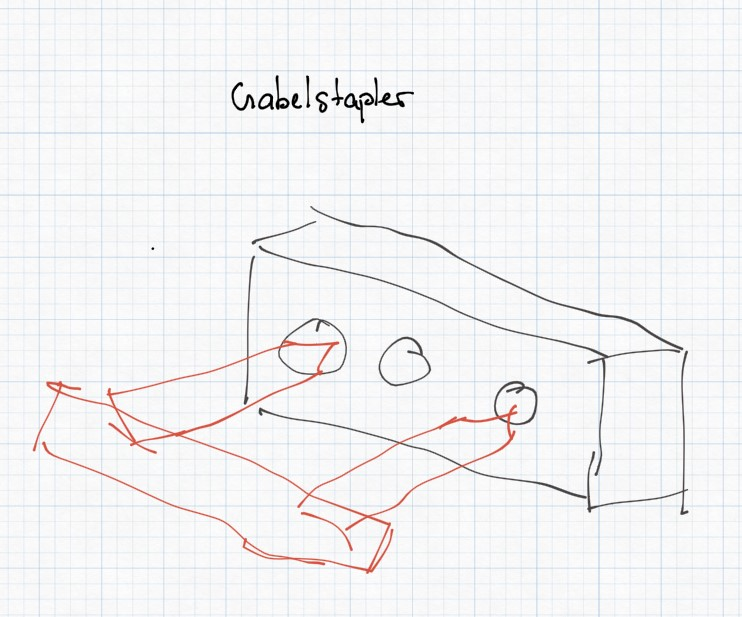
\includegraphics[width=\textwidth]{img/technologierecherche/Aufnahme/Gabelstapler.jpg}
        \caption{Prinzip angelehnt an einen Gabelstapler}
        \label{img:tech_Gaplerstapler}
    \end{minipage}
    \hfill
    \begin{minipage}{0.45\textwidth}
        \centering
        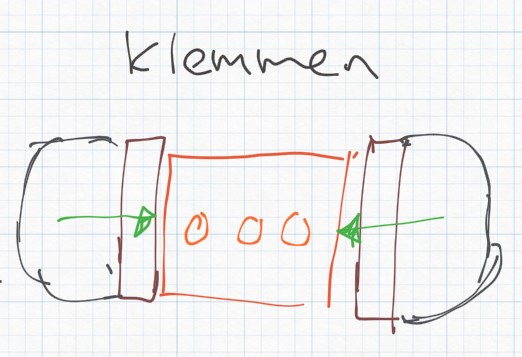
\includegraphics[width=\textwidth]{img/technologierecherche/Aufnahme/Laengsweg_Griff.jpg}
        \caption{Klemme über Längsweg des Hindernisses}
        \label{img:tech_Laengsweg_Griff}
    \end{minipage}
\end{figure}
\newpage
\begin{figure}[h!]
    \centering
    \begin{minipage}{0.45\textwidth}
        \centering
        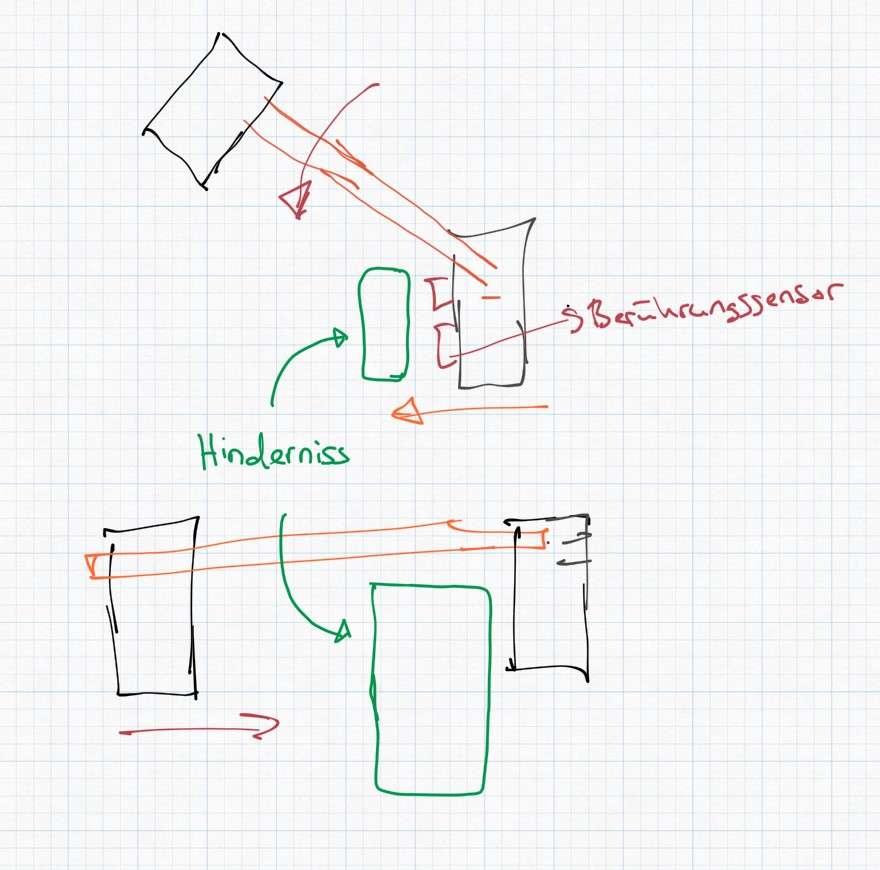
\includegraphics[width=\textwidth]{img/technologierecherche/Aufnahme/Breiterweg_Griff.jpg}
        \caption{Klemme über Breitenweg des Hindernisses, kann modifiziert werden, um Berührungssensoren zu verwenden}
        \label{img:tech_Breiterweg_Griff}
    \end{minipage}
    \hfill
    \begin{minipage}{0.45\textwidth}
        \centering
        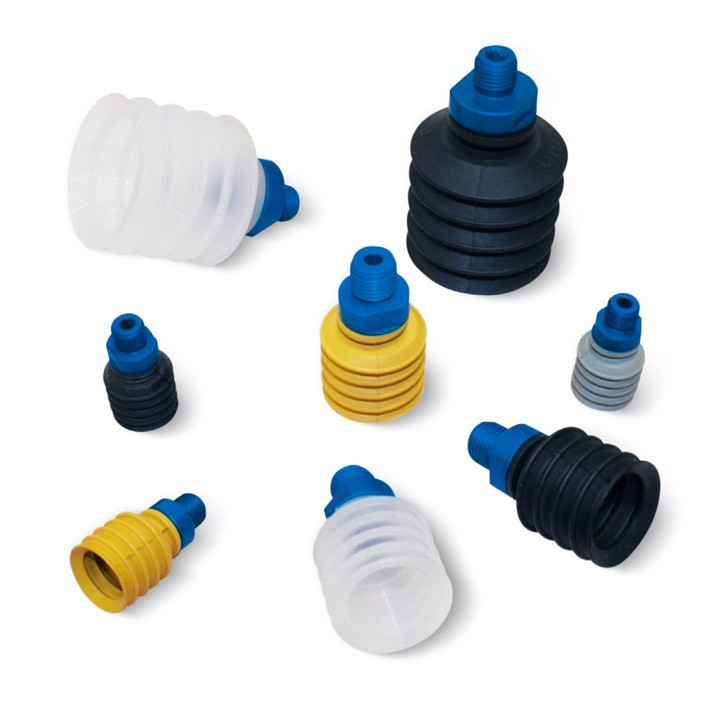
\includegraphics[width=\textwidth]{img/technologierecherche/Aufnahme/Vakuumgreifer.jpg}
        \caption{Aufnahme über Vakuumgreifer, Quelle: https://www.youtube.com/shorts/alxwWgzSVss} 
        \label{img:tech_Vakuumgreifer}
    \end{minipage}
\end{figure}


\newpage
\subsubsection{Rotation / Transport}
\begin{figure}[h!]
    \centering
    \begin{minipage}{0.45\textwidth}
        \centering
        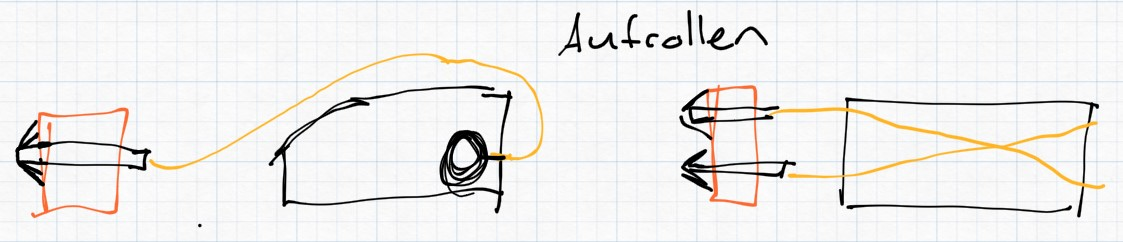
\includegraphics[width=\textwidth]{img/technologierecherche/Rotation/harponne.jpg}
        \caption{Eine Harpune artige Konstruktion, die die Löcher des Hindernisses ausnutzt}
        \label{img:tech_harponne}
    \end{minipage}
    \hfill
    \begin{minipage}{0.45\textwidth}
        \centering
        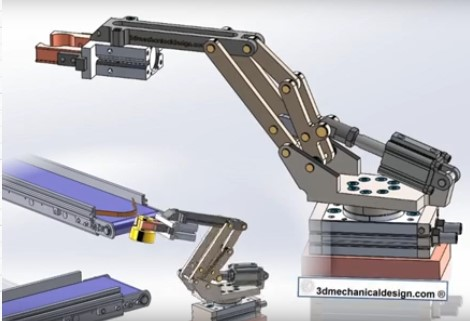
\includegraphics[width=\textwidth]{img/technologierecherche/Rotation/kran.jpg}
        \caption{Eine an einen Kran angelegte Konstruktion, Quelle: https://www.youtube.com/watch?v=VZRFHJfUkq4\&feature=youtu.be} 
        \label{img:tech_kran}
    \end{minipage}
\end{figure}

\begin{figure}[h!]
    \centering
    \begin{minipage}{0.45\textwidth}
        \centering
        \includegraphics[width=\textwidth]{img/technologierecherche/Rotation/seitlich_mit_räder.jpg}
        \caption{Für die Rotation wird das ganze Fahrzeug gewendet}
        \label{img:tech_seitlich_mit_räder}
    \end{minipage}
    \hfill
    \begin{minipage}{0.45\textwidth}
        \centering
        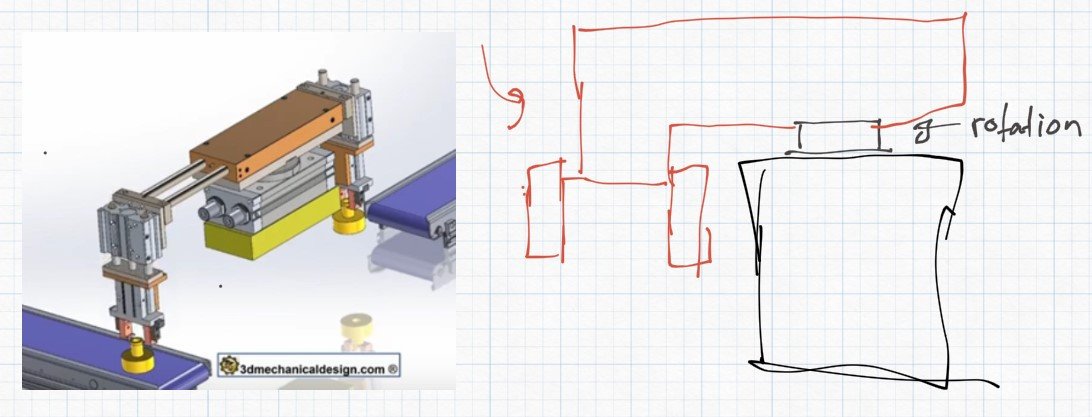
\includegraphics[width=\textwidth]{img/technologierecherche/Rotation/seitlich_mit_rotation.jpg}
        \caption{Ebenfalls an einen Kran angelegt, jedoch wird die Aufnahme von oben auf die Breite des Fahrzeuges durchgeführt, Quelle:https://www.youtube.com/watch?v=J7LGSNhFTU4} 
        \label{img:tech_seitlich_mit_rotation}
    \end{minipage}
\end{figure}
\newpage
\begin{figure}[h!]
    \centering
    \begin{minipage}{0.45\textwidth}
        \centering
        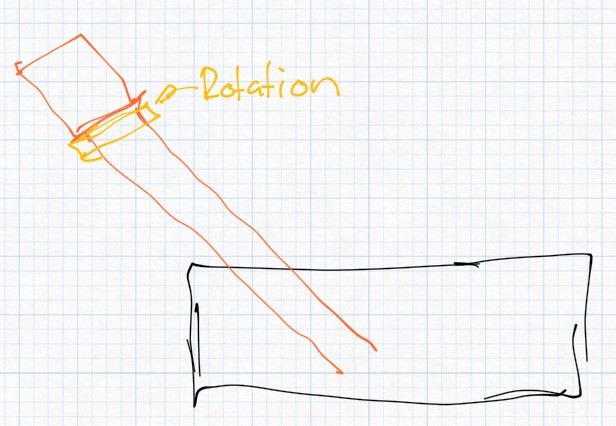
\includegraphics[width=\textwidth]{img/technologierecherche/Rotation/ueberkopf_griff_gelagert.jpg}
        \caption{}
        \label{img:tech_ueberkopf_griff_gelagert}
    \end{minipage}
    \hfill
    \begin{minipage}{0.45\textwidth}
        \centering
        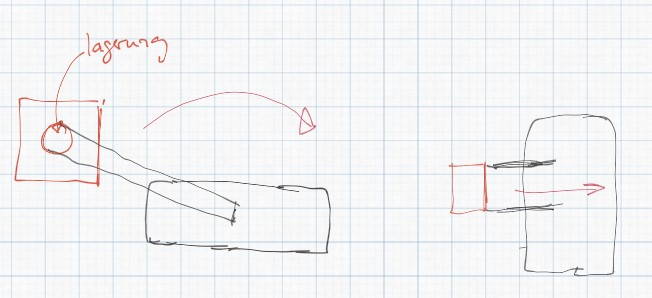
\includegraphics[width=\textwidth]{img/technologierecherche/Rotation/ueberkopf_objekt_gelagert.jpg}
        \caption{} 
        \label{img:tech_ueberkopf_objekt_gelagert}
    \end{minipage}
\end{figure}

\begin{figure}[h!]
    \centering
    \begin{minipage}{0.45\textwidth}
        \centering
        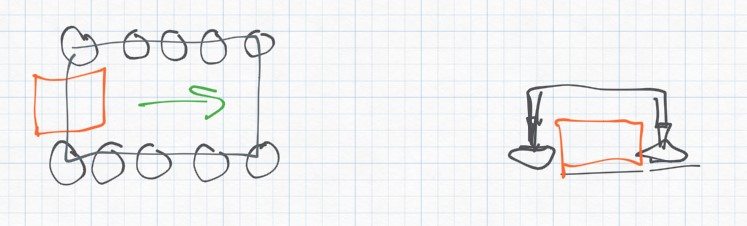
\includegraphics[width=\textwidth]{img/technologierecherche/Rotation/waescheanlage.jpg}
        \caption{}
        \label{img:tech_waescheanlage}
    \end{minipage}
    \hfill
    \begin{minipage}{0.45\textwidth}
        \centering
        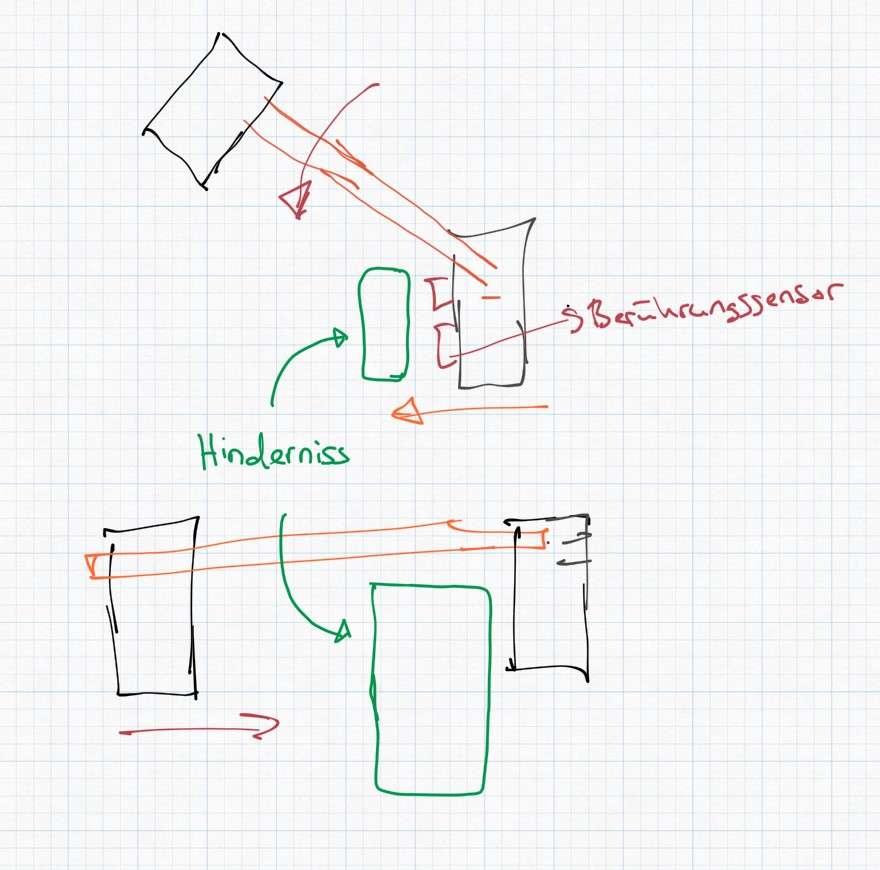
\includegraphics[width=\textwidth]{img/technologierecherche/Aufnahme/Breiterweg_Griff.jpg}
        \caption{} 
        \label{img:tech_nichts}
    \end{minipage}
\end{figure}
